%=====================================================================
%  Outer Measures, Pre-Measures, and Product Measures
%  Andrew Hwang
%
%  Expository notes reconstructed from the slides of the same talk.
%  Compile with: pdflatex measures.tex  (run twice for cross-refs)
%=====================================================================
\documentclass[11pt]{article}

\usepackage[margin=1.15in]{geometry}
\usepackage{amsmath,amssymb,amsthm}
\usepackage{mathtools}
\usepackage{enumitem}
\usepackage{float}
\usepackage{tikz}
\usetikzlibrary{calc,decorations.pathmorphing}
\usepackage[colorlinks=true,linkcolor=black,citecolor=black,urlcolor=blue]{hyperref}

\theoremstyle{definition}
\newtheorem{definition}{Definition}[section]
\newtheorem{example}[definition]{Example}
\newtheorem{remark}[definition]{Remark}

\theoremstyle{plain}
\newtheorem{theorem}[definition]{Theorem}
\newtheorem{proposition}[definition]{Proposition}
\newtheorem{lemma}[definition]{Lemma}
\newtheorem{corollary}[definition]{Corollary}

\newcommand{\R}{\mathbb{R}}
\newcommand{\Q}{\mathbb{Q}}
\newcommand{\Z}{\mathbb{Z}}
\newcommand{\Rbar}{\overline{\mathbb{R}}}
\newcommand{\M}{\mathcal{M}}
\newcommand{\N}{\mathcal{N}}
\newcommand{\A}{\mathcal{A}}
\newcommand{\B}{\mathcal{B}}
\newcommand{\Pow}{\mathcal{P}}
\newcommand{\Rect}{\mathfrak{R}}
\newcommand{\ostar}{\mu^{*}}
\DeclareMathOperator{\len}{length}

\title{\textbf{Outer Measures, Pre-Measures, and Product Measures}}
\author{Andrew Hwang\thanks{Notes from a talk given at Columbia Summer Learning Seminar, 08/18/2026.}}
\date{}

\begin{document}

\maketitle

\begin{abstract}
\noindent
We have gone over the development of the Lebesgue measure by beginning
with elementary notions of length and volume and extending them to more
complicated sets through coverings and outer measure. In these notes we
revisit that construction from a more general perspective. We introduce
the Carath\'eodory Extension Theorem, which recovers countable
additivity on a distinguished $\sigma$-algebra, and the
Hahn--Kolmogorov Extension Theorem, which builds an outer measure from
a premeasure on an algebra; together these are the ways we generate
measures. Using these extension theorems we explore
Lebesgue--Stieltjes measures and how different choices of increasing
right-continuous functions give rise to different measures on the Borel
$\sigma$-algebra. As an application we examine the Cantor set, which is
uncountable yet has measure zero, showing that cardinality and measure
are independent notions of size. From here, we also explore product
spaces and their respective product measures, along with the theory of
sections, leading into the Fubini--Tonelli theorems.
\end{abstract}

\tableofcontents

%=====================================================================
\section{Goal}
%=====================================================================

We know how to measure intervals and boxes on the real line using the
Lebesgue measure. But there are many other types of measures. The idea
of this talk is to discuss how we construct general measures beyond the
Lebesgue measure.

%---------------------------------------------------------------------
\subsection{Recall: \texorpdfstring{$\sigma$}{sigma}-Algebras and Measures}
%---------------------------------------------------------------------

\begin{definition}[$\sigma$-algebra]
A collection $\M$ of subsets of a set $X$ is a \emph{$\sigma$-algebra}
if:
\begin{enumerate}[label=\arabic*.]
  \item $\emptyset \in \M$ (and hence $X \in \M$);
  \item $A \in \M \implies A^{c} \in \M$ (closed under complements);
  \item $A_1, A_2, \ldots \in \M \implies \bigcup_{j=1}^{\infty} A_j \in \M$
        (closed under countable unions).
\end{enumerate}
\end{definition}

\begin{definition}[Measure]
A function $\mu : \M \to [0,\infty]$ is a \emph{measure} if:
\begin{enumerate}[label=\arabic*.]
  \item $\mu(\emptyset) = 0$;
  \item for any countable collection $\{A_j\}_{j=1}^{\infty} \subset \M$
        of \emph{pairwise disjoint} sets,
        \[
          \mu\left( \bigcup_{j=1}^{\infty} A_j \right)
            \;=\; \sum_{j=1}^{\infty} \mu(A_j)
        \]
        (countable additivity).
\end{enumerate}
\end{definition}

%=====================================================================
\section{Outer Measures}
%=====================================================================

An \emph{outer measure} is a function
\[
  \ostar : 2^{X} \longrightarrow [0,\infty]
\]
satisfying:
\begin{enumerate}[label=\arabic*.]
  \item $\ostar(\emptyset) = 0$;
  \item if $A \subseteq B$, then $\ostar(A) \le \ostar(B)$;
  \item given a countable collection of sets $\{A_i\}_{i=1}^{\infty}$,
        we have that
        \[
          \ostar\left( \bigcup_{i=1}^{\infty} A_i \right)
            \;\le\; \sum_{i=1}^{\infty} \ostar(A_i).
        \]
\end{enumerate}

Note the two ways in which this is weaker than a measure: the domain is
all of the power set rather than a $\sigma$-algebra, and countable
additivity has been relaxed to countable \emph{sub}additivity. The
first is what makes outer measures easy to build; the second is the
price we pay, and the rest of this section is about recovering
additivity on a suitable subfamily of sets.

%---------------------------------------------------------------------
\subsection{Carath\'eodory Measurability}
%---------------------------------------------------------------------

\begin{definition}[Carath\'eodory measurable]
We say that a set $A \in \Pow(X)$ is \emph{Carath\'eodory measurable}
(or just \emph{$\ostar$-measurable}) if for all $E \in \Pow(X)$ we have
that
\[
  \ostar(E) \;=\; \ostar(E \cap A) + \ostar(E \setminus A).
\]
\end{definition}

The condition says that $A$ splits every test set $E$ additively.
Subadditivity already gives $\ostar(E) \le \ostar(E \cap A) +
\ostar(E \setminus A)$ for free, so the content of the definition is
always the reverse inequality.

\begin{figure}[H]
\centering
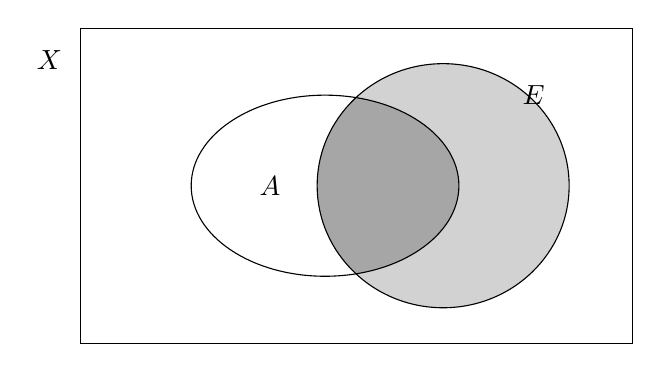
\begin{tikzpicture}[scale=1.0]
  \draw (0,0) rectangle (7,4);
  \node at (-0.4,3.6) {$X$};
  \fill[gray!35] (4.6,2) ellipse (1.6 and 1.55);
  \begin{scope}
    \clip (4.6,2) ellipse (1.6 and 1.55);
    \fill[gray!70] (3.1,2) ellipse (1.7 and 1.15);
  \end{scope}
  \draw (3.1,2) ellipse (1.7 and 1.15);
  \draw (4.6,2) ellipse (1.6 and 1.55);
  \node at (2.4,2) {$A$};
  \node at (5.75,3.15) {$E$};
\end{tikzpicture}
\caption{Carath\'eodory's splitting condition: $A$ cuts the test set
$E$ into $E \cap A$ and $E \setminus A$, and the two outer measures
must add back up to $\ostar(E)$.}
\end{figure}

\begin{example}[Null sets]
Given some space $X$ and a null set $E$ (that is, $\ostar(E) = 0$), we
can see that for some arbitrary $B \in \Pow(X)$ we have
$\ostar(B \cap E) + \ostar(B \setminus E) \ge \ostar(B)$ because of
countable subadditivity. Moreover, we can see that since
$B \cap E \subseteq E$, by monotonicity $\ostar(B \cap E) \le
\ostar(E) = 0$. Similarly, we can say that $B \setminus E \subseteq B$,
so $\ostar(B \setminus E) \le \ostar(B)$. Hence we have
\[
  \ostar(B \cap E) + \ostar(B \setminus E)
    \;\le\; 0 + \ostar(B) \;=\; \ostar(B).
\]
Therefore $\ostar(B \cap E) + \ostar(B \setminus E) = \ostar(B)$, so
every null set is Carath\'eodory measurable.
\end{example}

%---------------------------------------------------------------------
\subsection{The Measurable Sets Form a \texorpdfstring{$\sigma$}{sigma}-Algebra}
%---------------------------------------------------------------------

Let $\B = \{ A \in \Pow(X) : A \text{ is } \ostar\text{-measurable} \}$.
Then $\B$ is a $\sigma$-algebra on $X$.

\begin{itemize}
  \item \textbf{$\emptyset, X \in \B$:}
        $\ostar(E \cap \emptyset) + \ostar(E \setminus \emptyset)
          = 0 + \ostar(E)$.
  \item \textbf{Closed under complements:} the condition
        $\ostar(E) = \ostar(E \cap A) + \ostar(E \setminus A)$ is
        symmetric in $A$ and $A^{c}$, since $E \cap A^{c} =
        E \setminus A$ and $E \setminus A^{c} = E \cap A$. So
        $A \in \B \iff A^{c} \in \B$, for free.
  \item \textbf{Closed under countable unions:} apply the definition
        twice to get $A \cup B \in \B$, then disjointify
        $\bigcup_{i=1}^{\infty} A_i$ and pass to the limit.
\end{itemize}

%---------------------------------------------------------------------
\subsection{Carath\'eodory's Extension Theorem}
%---------------------------------------------------------------------

\begin{theorem}[Carath\'eodory]
Given an outer measure $\ostar : 2^{X} \to [0,\infty]$ and
$\B = \{ E : E \in \Pow(X) \text{ and } E \text{ is }
\ostar\text{-measurable} \}$, the restriction of $\ostar$ onto $\B$ is a
measure and $\B$ is a $\sigma$-algebra. That is, $\ostar|_{\B} = \mu$
and $\mu(A) = \ostar(A)$ if $A \in \B$.
\end{theorem}

The main results are:
\begin{itemize}
  \item $\B$ is a $\sigma$-algebra;
  \item $\ostar|_{\B}$ is a measure;
  \item starting from an outer measure defined on the power set, we can
        restrict the domain to create a measure.
\end{itemize}

%=====================================================================
\section{Pre-Measures and the Hahn--Kolmogorov Theorem}
%=====================================================================

Carath\'eodory's theorem takes an outer measure as input. The next
question is where outer measures come from. The answer is that they can
be manufactured by covering, starting from a set function defined only
on a much smaller and more concrete family of sets.

%---------------------------------------------------------------------
\subsection{Algebras (Boolean Algebras)}
%---------------------------------------------------------------------

\begin{definition}[Algebra]
Given a set $X$, an \emph{algebra} $\A$ on $X$ is a collection of
subsets of $X$ such that
\begin{itemize}
  \item $X \in \A$;
  \item if $A \in \A$, then $A^{c} \in \A$, where the complement is
        taken relative to $X$;
  \item if $\{A_i\}_{i=1}^{n} \subseteq \A$, then
        \[
          \bigcup_{i=1}^{n} A_i \in \A.
        \]
\end{itemize}
\end{definition}

So an algebra is a $\sigma$-algebra with countable unions weakened to
finite unions.

%---------------------------------------------------------------------
\subsection{Pre-Measures}
%---------------------------------------------------------------------

\begin{definition}[Pre-measure]
Given a set $X$ and an algebra $\A$ on $X$, a \emph{premeasure} is a
function
\[
  \mu_0 : \A \to [0,\infty]
\]
such that
\begin{itemize}
  \item $\mu_0(\emptyset) = 0$;
  \item if $\{A_i\}_{i=1}^{\infty} \subseteq \A$ is a countable
        collection of pairwise disjoint sets and
        \[
          \bigcup_{i=1}^{\infty} A_i \in \A,
        \]
        then
        \[
          \mu_0\left( \bigcup_{i=1}^{\infty} A_i \right)
            \;=\; \sum_{i=1}^{\infty} \mu_0(A_i).
        \]
\end{itemize}
\end{definition}

The countable additivity requirement is conditional: it is imposed only
when the countable union happens to land back inside $\A$, which for an
algebra is not automatic.

%---------------------------------------------------------------------
\subsection{The Hahn--Kolmogorov Theorem}
%---------------------------------------------------------------------

\begin{theorem}[Hahn--Kolmogorov]
Let $\A \subseteq \Pow(X)$ be an algebra and $\mu_0 : \A \to [0,\infty]$
a premeasure. For $E \in \Pow(X)$, define
\[
  \ostar(E) \;=\;
    \inf\left\{ \sum_{i=1}^{\infty} \mu_0(A_i)
      \;:\; A_i \in \A, \; E \subseteq \bigcup_{i=1}^{\infty} A_i \right\}.
\]
Then $\ostar$ is an outer measure on $X$.
\end{theorem}

\noindent
\textbf{Then apply Carath\'eodory.} Let
$\B = \{ A \in \Pow(X) : A \text{ is } \ostar\text{-measurable} \}$.
Then $\B$ is a $\sigma$-algebra and $\ostar|_{\B}$ is a measure.

%---------------------------------------------------------------------
\subsection{Where the Resulting Measure Lives}
%---------------------------------------------------------------------

The two theorems chain together. One shows that $\A \subseteq \B$; then
\[
  \A \subseteq \B
  \quad \overset{\B \text{ is a } \sigma\text{-algebra}}{\Longrightarrow} \quad
  \sigma(\A) \subseteq \B
  \quad \overset{\ostar|_{\B} \text{ is a measure}}{\Longrightarrow} \quad
  \ostar|_{\sigma(\A)} \text{ is a measure},
\]
and altogether
\[
  \A \;\subseteq\; \sigma(\A) \;\subseteq\; \B \;\subseteq\; \Pow(X).
\]

%---------------------------------------------------------------------
\subsection{Carath\'eodory vs.\ Hahn--Kolmogorov}
%---------------------------------------------------------------------

The two inclusions $\sigma(\A) \subseteq \B$ are typically strict, and
the gap is not a technicality. In the case of Lebesgue measure on $\R$,
$\sigma(\A)$ is the Borel $\sigma$-algebra while $\B$ is the strictly
larger $\sigma$-algebra of Lebesgue measurable sets --- the
Carath\'eodory construction automatically includes every null set,
whereas the Borel sets do not.

\begin{figure}[H]
\centering
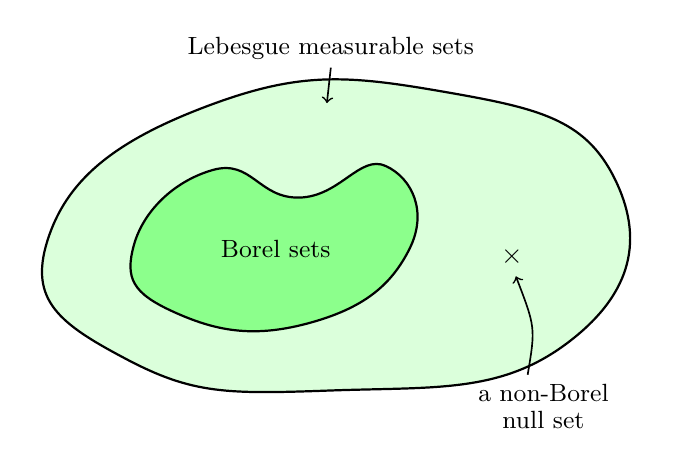
\begin{tikzpicture}[scale=1.0]
  \fill[green!14]
    plot[smooth cycle,tension=0.85] coordinates
      {(0,0.2) (2,1.9) (5,2.1) (7.2,1.0) (6.6,-1.1) (3.6,-1.7) (1.0,-1.3)};
  \draw[line width=0.8pt]
    plot[smooth cycle,tension=0.85] coordinates
      {(0,0.2) (2,1.9) (5,2.1) (7.2,1.0) (6.6,-1.1) (3.6,-1.7) (1.0,-1.3)};
  \fill[green!45]
    plot[smooth cycle,tension=0.85] coordinates
      {(1.1,0.15) (2.1,1.1) (3.2,0.75) (4.3,1.15) (4.6,0.1) (3.3,-0.85) (1.6,-0.7)};
  \draw[line width=0.8pt]
    plot[smooth cycle,tension=0.85] coordinates
      {(1.1,0.15) (2.1,1.1) (3.2,0.75) (4.3,1.15) (4.6,0.1) (3.3,-0.85) (1.6,-0.7)};
  \node at (2.9,0.1) {\small Borel sets};
  \node at (3.6,2.65) {\small Lebesgue measurable sets};
  \draw[->,line width=0.6pt] (3.6,2.4) -- (3.55,1.95);
  \node at (5.9,0.0) {$\times$};
  \node[align=center] at (6.3,-1.9) {\small a non-Borel\\[-2pt] \small null set};
  \draw[->,line width=0.6pt] (6.1,-1.5) .. controls (6.2,-0.9) .. (5.95,-0.25);
\end{tikzpicture}
\caption{The Lebesgue measurable sets properly contain the Borel sets.}
\end{figure}

%=====================================================================
\section{Borel and Lebesgue--Stieltjes Measures}
%=====================================================================

Using what we have developed, we can now construct Borel measures and,
specifically, Lebesgue--Stieltjes measures.

Let $F : \R \to \R$ be \textbf{increasing} and \textbf{right-continuous}.

Let $\A$ be the collection of finite disjoint unions of half-open
intervals $(a,b]$, where $-\infty \le a \le b \le \infty$. Then $\A$ is
an algebra and
\[
  \sigma(\A) \;=\; \B_{\R}.
\]

Define $\mu_0 : \A \to [0,\infty]$ by
\[
  \mu_0\big((a,b]\big) \;=\; F(b) - F(a),
  \qquad
  \mu_0\left( \bigsqcup_{i=1}^{n} (a_i,b_i] \right)
    \;=\; \sum_{i=1}^{n} \big( F(b_i) - F(a_i) \big).
\]

%---------------------------------------------------------------------
\subsection{Lebesgue--Stieltjes Measures}
%---------------------------------------------------------------------

By Hahn--Kolmogorov, $\mu_0$ extends to a measure $\mu_F$ on $\B_{\R}$
with
\[
  \mu_F\big((a,b]\big) \;=\; F(b) - F(a).
\]
We call $\mu_F$ the \textbf{Lebesgue--Stieltjes measure} of $F$.

Taking $F(x) = x$:
\[
  \mu_F\big((a,b]\big) \;=\; b - a \;=\; \lambda\big((a,b]\big).
\]
So Lebesgue measure is the Lebesgue--Stieltjes measure of the identity.
Other choices of $F$ recover other familiar measures:

\begin{center}
\begin{tabular}{ll}
  $F(x) = x$ & Lebesgue measure $\lambda$ \\[2pt]
  $F = \mathbf{1}_{[0,\infty)}$ & Dirac measure $\delta_0$ \\[2pt]
  $F(x) = \lfloor x \rfloor$ & counting measure on $\Z$
\end{tabular}
\end{center}

%=====================================================================
\section{An Application: The Cantor Set}
%=====================================================================

%---------------------------------------------------------------------
\subsection{The Question}
%---------------------------------------------------------------------

We have now formally defined the construction of the Lebesgue measure
as well as other Lebesgue--Stieltjes measures. From this, we have the
following results under the standard Lebesgue measure $m$:
\begin{itemize}
  \item $m(\Q) = 0$;
  \item $m((0,1)) = 1$;
  \item $m(\R) = \infty$;
  \item $m((0,1) \setminus \Q) = 1$.
\end{itemize}

We can see that the measure of uncountable sets like the interval
$(0,1)$ or the reals is positive. Then, is the measure of uncountable
sets always positive?

%---------------------------------------------------------------------
\subsection{The Cantor Set}
%---------------------------------------------------------------------

We construct the Cantor set $C \subset [0,1]$ by successively removing
open middle thirds. Let
\[
  C_0 = [0,1].
\]
Remove the open middle third to get
\[
  C_1 = \left[0,\tfrac{1}{3}\right] \cup \left[\tfrac{2}{3},1\right].
\]
Remove the open middle third of each remaining interval to get
\[
  C_2 = \left[0,\tfrac{1}{9}\right] \cup \left[\tfrac{2}{9},\tfrac{1}{3}\right]
        \cup \left[\tfrac{2}{3},\tfrac{7}{9}\right] \cup \left[\tfrac{8}{9},1\right],
\]
and so on: at stage $n$, $C_n$ consists of $2^{n}$ closed intervals,
each of length $3^{-n}$. The Cantor set is defined as
\[
  C \;=\; \bigcap_{n=0}^{\infty} C_n.
\]

\begin{figure}[H]
\centering
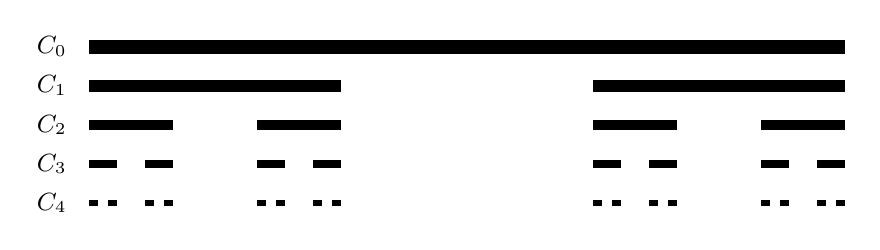
\begin{tikzpicture}[scale=0.8]
  \draw[line width=5.20pt] (0.0000,-0.000) -- (12.0000,-0.000);
  \draw[line width=4.45pt] (0.0000,-0.620) -- (4.0000,-0.620);
  \draw[line width=3.70pt] (0.0000,-1.240) -- (1.3333,-1.240);
  \draw[line width=2.95pt] (0.0000,-1.860) -- (0.4444,-1.860);
  \draw[line width=2.20pt] (0.0000,-2.480) -- (0.1481,-2.480);
  \draw[line width=2.20pt] (0.2963,-2.480) -- (0.4444,-2.480);
  \draw[line width=2.95pt] (0.8889,-1.860) -- (1.3333,-1.860);
  \draw[line width=2.20pt] (0.8889,-2.480) -- (1.0370,-2.480);
  \draw[line width=2.20pt] (1.1852,-2.480) -- (1.3333,-2.480);
  \draw[line width=3.70pt] (2.6667,-1.240) -- (4.0000,-1.240);
  \draw[line width=2.95pt] (2.6667,-1.860) -- (3.1111,-1.860);
  \draw[line width=2.20pt] (2.6667,-2.480) -- (2.8148,-2.480);
  \draw[line width=2.20pt] (2.9630,-2.480) -- (3.1111,-2.480);
  \draw[line width=2.95pt] (3.5556,-1.860) -- (4.0000,-1.860);
  \draw[line width=2.20pt] (3.5556,-2.480) -- (3.7037,-2.480);
  \draw[line width=2.20pt] (3.8519,-2.480) -- (4.0000,-2.480);
  \draw[line width=4.45pt] (8.0000,-0.620) -- (12.0000,-0.620);
  \draw[line width=3.70pt] (8.0000,-1.240) -- (9.3333,-1.240);
  \draw[line width=2.95pt] (8.0000,-1.860) -- (8.4444,-1.860);
  \draw[line width=2.20pt] (8.0000,-2.480) -- (8.1481,-2.480);
  \draw[line width=2.20pt] (8.2963,-2.480) -- (8.4444,-2.480);
  \draw[line width=2.95pt] (8.8889,-1.860) -- (9.3333,-1.860);
  \draw[line width=2.20pt] (8.8889,-2.480) -- (9.0370,-2.480);
  \draw[line width=2.20pt] (9.1852,-2.480) -- (9.3333,-2.480);
  \draw[line width=3.70pt] (10.6667,-1.240) -- (12.0000,-1.240);
  \draw[line width=2.95pt] (10.6667,-1.860) -- (11.1111,-1.860);
  \draw[line width=2.20pt] (10.6667,-2.480) -- (10.8148,-2.480);
  \draw[line width=2.20pt] (10.9630,-2.480) -- (11.1111,-2.480);
  \draw[line width=2.95pt] (11.5556,-1.860) -- (12.0000,-1.860);
  \draw[line width=2.20pt] (11.5556,-2.480) -- (11.7037,-2.480);
  \draw[line width=2.20pt] (11.8519,-2.480) -- (12.0000,-2.480);
  \node[left] at (-0.2,-0.000) {\small $C_0$};
  \node[left] at (-0.2,-0.620) {\small $C_1$};
  \node[left] at (-0.2,-1.240) {\small $C_2$};
  \node[left] at (-0.2,-1.860) {\small $C_3$};
  \node[left] at (-0.2,-2.480) {\small $C_4$};
\end{tikzpicture}
\caption{The first five stages of the middle-thirds construction.}
\end{figure}

\begin{remark}[Measure of $C$]
Each $C_n$ is a finite union of $2^n$ closed intervals of length
$3^{-n}$, so $m(C_n) = (2/3)^{n}$. Since $C \subseteq C_n$ for every
$n$, monotonicity gives $m(C) \le (2/3)^{n} \to 0$, and therefore
$m(C) = 0$. Each $C_n$ is closed, so $C$ is closed as well.
\end{remark}

%---------------------------------------------------------------------
\subsection{Every Point of \texorpdfstring{$C$}{C} is a Limit Point}
%---------------------------------------------------------------------

Let $x \in C$. For each $n$, let $I_n$ be the unique interval of $C_n$
containing $x$, so
\[
  \len(I_n) = 3^{-n}, \qquad I_0 \supset I_1 \supset I_2 \supset \cdots.
\]
Let $x_n$ be an endpoint of $I_n$ with $x_n \ne x$. Endpoints of
$C_n$-intervals are never removed later, so $x_n \in C$ for all $n$.
Since $x_n, x \in I_n$,
\[
  |x_n - x| \;\le\; \len(I_n) \;=\; 3^{-n} \;\to\; 0,
\]
so $x_n \to x$ with $x_n \ne x$. Hence $x$ is a limit point of $C$.

\begin{corollary}
$C$ is uncountable. (In general, every nonempty perfect subset of a
complete metric space is uncountable: no countable set can be perfect,
since one can always find, inductively, a nested sequence of closed
balls avoiding each listed point in turn, and by completeness their
intersection is nonempty and contains a point not on the list.)
\end{corollary}

\begin{remark}[Cardinality vs.\ measure]
It is worth pausing on how strange this is. The Cantor set $C$
satisfies
\[
  |C| = |\R| = |(0,1)|,
\]
i.e.\ $C$ has the same cardinality as the entire real line --- it is
``just as large'' as $(0,1)$ in the sense of counting points. And yet
\[
  m(C) = 0,
\]
while $m((0,1)) = 1$. So $C$ is a set with the full cardinality of the
continuum, but zero length. This shows that cardinality and Lebesgue
measure are fundamentally different ways of measuring the ``size'' of a
set: a set can be uncountable --- even continuum-sized --- while still
being negligible from the point of view of measure.
\end{remark}

%=====================================================================
\section{Product Measures}
%=====================================================================

Naturally, we don't work in just one space. For instance, consider any
space with multiple coordinates, or joint distributions and their joint
CDFs. These all require taking the product of multiple different
measurable spaces.

Let us recall what the Cartesian product was. If we have two sets $A$
and $B$, the Cartesian product is defined as follows:
\[
  A \times B := \{ (a,b) : a \in A \text{ and } b \in B \}.
\]

Consider the product space $\R \times \R$. This is one of the simplest
and most common examples of a product space. More generally, we may
consider a product of spaces
\[
  \prod_{n} X_n.
\]

If we want to define a measure on such a product space, we must first
specify a $\sigma$-algebra of measurable subsets of that space. This
motivates the question: given $\sigma$-algebras on the individual
spaces, how should we construct a natural $\sigma$-algebra on their
product?

%---------------------------------------------------------------------
\subsection{The Product \texorpdfstring{$\sigma$}{sigma}-Algebra}
%---------------------------------------------------------------------

A very natural way we might think about what a $\sigma$-algebra of a
product space might be is the set of rectangles. For now, let us just
think of a product space of two measurable spaces $(X,\M)$ and
$(Y,\N)$. We define
\[
  \Rect := \{ A \times B : A \in \M \text{ and } B \in \N \}.
\]
So $\Rect$ seems like it would be a nice $\sigma$-algebra for our
product space; but, is it really a $\sigma$-algebra?

\begin{figure}[H]
\centering
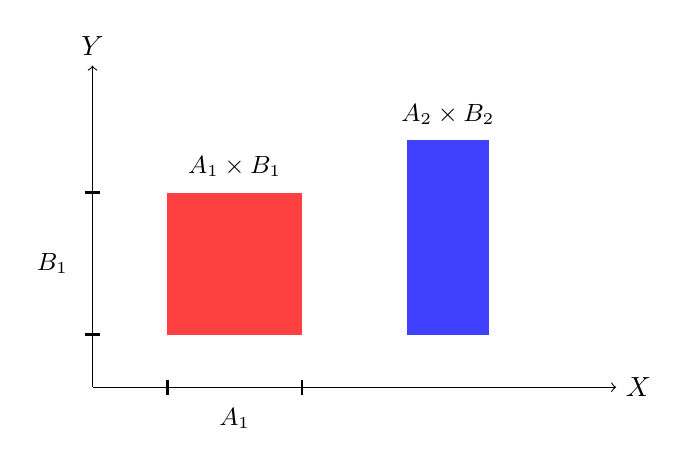
\begin{tikzpicture}[scale=0.95]
  \draw[->] (0,0) -- (7,0) node[right] {$X$};
  \draw[->] (0,0) -- (0,4.3) node[above] {$Y$};
  \fill[red!75] (1.0,0.7) rectangle (2.8,2.6);
  \node at (1.9,2.95) {\small $A_1 \times B_1$};
  \fill[blue!75] (4.2,0.7) rectangle (5.3,3.3);
  \node at (4.75,3.65) {\small $A_2 \times B_2$};
  \draw[line width=1pt] (1.0,-0.1) -- (1.0,0.1);
  \draw[line width=1pt] (2.8,-0.1) -- (2.8,0.1);
  \draw[line width=1pt] (-0.1,0.7) -- (0.1,0.7);
  \draw[line width=1pt] (-0.1,2.6) -- (0.1,2.6);
  \node[below] at (1.9,-0.15) {\small $A_1$};
  \node[left] at (-0.2,1.65) {\small $B_1$};
\end{tikzpicture}
\caption{Measurable rectangles in $X \times Y$.}
\end{figure}

It turns out that $\Rect$ is not a $\sigma$-algebra. Recall that one of
the requirements of a $\sigma$-algebra is that it must be closed under
complements. However, $\Rect$ contains only rectangles of the form
$A \times B$. In general, the complement of a rectangle is not itself a
rectangle, so it need not belong to $\Rect$. Thus, $\Rect$ is not
closed under complements and therefore is not a $\sigma$-algebra.

To fix this, we take the smallest $\sigma$-algebra containing all of
the rectangles in $\Rect$. That is, we define
\[
  \sigma(\Rect),
\]
the $\sigma$-algebra generated by $\Rect$. This is what we call the
\textbf{product $\sigma$-algebra}, and we write
\[
  \M \otimes \N := \sigma(\Rect).
\]

%---------------------------------------------------------------------
\subsection{Projection Maps}
%---------------------------------------------------------------------

Moreover, another very natural structure that arises from a product
space is the notion of a \textbf{projection map}. For example, given
the product space $X \times Y$, we have the two coordinate projections
\[
  \pi_1 : X \times Y \to X, \qquad \pi_1(x,y) = x,
\]
and
\[
  \pi_2 : X \times Y \to Y, \qquad \pi_2(x,y) = y.
\]
In other words, $\pi_1$ simply extracts the first coordinate of
$(x,y)$, while $\pi_2$ extracts the second coordinate. Since these
projection maps arise naturally from the product space, we would like
our product $\sigma$-algebra to make both $\pi_1$ and $\pi_2$
measurable.

Recall that a function
\[
  f : (S,\A) \to (T,\B)
\]
is measurable if, for every measurable set $E \in \B$, its preimage
$f^{-1}(E)$ belongs to $\A$. Therefore, for the first projection
$\pi_1$ to be measurable, we must have
\[
  \pi_1^{-1}(A)
\]
measurable in $X \times Y$ for every $A \in \M$. Similarly, for the
second projection $\pi_2$ to be measurable, we must have
\[
  \pi_2^{-1}(B)
\]
measurable in $X \times Y$ for every $B \in \N$. Thus, the smallest
$\sigma$-algebra on $X \times Y$ that makes both coordinate projections
measurable is the $\sigma$-algebra generated by all of these preimages:
\[
  \sigma\left( \{\pi_1^{-1}(A) : A \in \M\}
    \cup \{\pi_2^{-1}(B) : B \in \N\} \right).
\]

%---------------------------------------------------------------------
\subsection{The Two Descriptions Agree}
%---------------------------------------------------------------------

We will now show that this is exactly the same $\sigma$-algebra as the
one generated by the measurable rectangles. That is,
\[
  \M \otimes \N \;=\; \sigma(\Rect)
    \;=\; \sigma\left( \{\pi_1^{-1}(A) : A \in \M\}
      \cup \{\pi_2^{-1}(B) : B \in \N\} \right).
\]

For any $A \in \M$ and $B \in \N$,
\[
  \pi_1^{-1}(A) = A \times Y, \qquad \pi_2^{-1}(B) = X \times B.
\]
Thus, the preimages of the coordinate projections are themselves
measurable rectangles. Conversely, every measurable rectangle can be
written using these preimages:
\[
  A \times B = \pi_1^{-1}(A) \cap \pi_2^{-1}(B).
\]
Therefore, the measurable rectangles and the projection preimages
generate the same $\sigma$-algebra. Hence,
\[
  \boxed{\;\M \otimes \N \;=\; \sigma(\Rect)
    \;=\; \sigma\left( \{\pi_1^{-1}(A) : A \in \M\}
      \cup \{\pi_2^{-1}(B) : B \in \N\} \right).\;}
\]

%---------------------------------------------------------------------
\subsection{The Algebra of Finite Disjoint Unions}
%---------------------------------------------------------------------

Let $\A$ be the collection of \emph{finite disjoint unions} of
rectangles,
\[
  \A \;=\; \left\{ \bigsqcup_{i=1}^{n} (A_i \times B_i)
    \;:\; A_i \in \M, \; B_i \in \N \right\}.
\]
Then $\A$ is an algebra, and
\[
  \Rect \;\subseteq\; \A \;\subseteq\; \sigma(\Rect)
    \;=\; \sigma(\A) \;=\; \M \otimes \N.
\]

Now apply ``$\mathcal{C} \subseteq \sigma(\mathcal{D}) \implies
\sigma(\mathcal{C}) \subseteq \sigma(\mathcal{D})$'' in both directions:
\begin{itemize}
  \item $\Rect \subseteq \A \subseteq \sigma(\A)$, so
        $\sigma(\Rect) \subseteq \sigma(\A)$;
  \item $\A \subseteq \sigma(\Rect)$, so
        $\sigma(\A) \subseteq \sigma(\Rect)$.
\end{itemize}

%---------------------------------------------------------------------
\subsection{Constructing the Product Measure}
%---------------------------------------------------------------------

\noindent
\textbf{Goal.} The most natural requirement we want is that for a
``clean'' rectangle $A \times B$ with $A \in \M$, $B \in \N$, the
product measure should satisfy
\[
  (\mu \times \nu)(A \times B) = \mu(A)\,\nu(B).
\]

\medskip
\noindent
\textbf{Step 1: The algebra of rectangles.} Let $\A$ be the collection
of all \emph{finite disjoint unions} of rectangles $A \times B$ with
$A \in \M$, $B \in \N$. One checks that $\A$ is an algebra: it is
closed under complements and finite unions, and every $E \in \A$ can be
written as
\[
  E = \bigsqcup_{j=1}^{n} A_j \times B_j
\]
for some finite collection of pairwise disjoint rectangles
$A_j \times B_j$.

\medskip
\noindent
\textbf{Step 2: A premeasure on $\A$.} Define
$\pi : \A \to [0,\infty]$ by
\[
  \pi(E) = \sum_{j=1}^{n} \mu(A_j)\,\nu(B_j)
  \qquad \text{where } E = \bigsqcup_{j=1}^{n} A_j \times B_j.
\]

\medskip
\noindent
\textbf{Step 3: Hahn--Kolmogorov extension.} Define an outer measure
$\pi^{*}$ on all of $X \times Y$ by
\[
  \pi^{*}(E) = \inf\left\{ \sum_{j=1}^{\infty} \pi(E_j)
    \;:\; E \subset \bigcup_{j=1}^{\infty} E_j, \; E_j \in \A \right\}.
\]
By the Carath\'eodory extension theorem, the restriction of $\pi^{*}$
to the $\sigma$-algebra $\M \otimes \N$ generated by $\A$ is a genuine
measure, and it agrees with $\pi$ on $\A$.

\begin{definition}[Product measure]
We call this resulting measure the \emph{product measure}, denoted
$\mu \times \nu$, on $(X \times Y, \M \otimes \N)$. In particular,
\[
  (\mu \times \nu)(A \times B) = \mu(A)\,\nu(B)
\]
for all $A \in \M$, $B \in \N$, as desired.
\end{definition}

%---------------------------------------------------------------------
\subsection{Is It Well-Defined?}
%---------------------------------------------------------------------

A set $E \in \A$ may be written as a finite disjoint union of
rectangles in more than one way, so we must check that $\pi(E)$ does
not depend on the decomposition chosen.

\begin{proposition}
Suppose $A \times B$ is a rectangle that is a (finite or countable)
disjoint union of rectangles $A_j \times B_j$. Then for $x \in X$ and
$y \in Y$,
\[
  \chi_A(x)\chi_B(y) = \chi_{A \times B}(x,y)
    = \sum_j \chi_{A_j \times B_j}(x,y)
    = \sum_j \chi_{A_j}(x)\chi_{B_j}(y).
\]
\end{proposition}

Integrating both sides and applying the monotone convergence theorem to
interchange the sum and the integrals:
\begin{align*}
  \int_X \int_Y \chi_A(x)\chi_B(y) \,d\nu(y)\,d\mu(x)
    &= \int_X \int_Y \sum_j \chi_{A_j}(x)\chi_{B_j}(y) \,d\nu(y)\,d\mu(x) \\[4pt]
  \int_X \chi_A(x) \left( \int_Y \chi_B(y) \,d\nu(y) \right) d\mu(x)
    &= \int_X \sum_j \chi_{A_j}(x)
       \left( \int_Y \chi_{B_j}(y) \,d\nu(y) \right) d\mu(x) \\[4pt]
  \int_X \chi_A(x)\,\nu(B) \,d\mu(x)
    &= \int_X \sum_j \chi_{A_j}(x)\,\nu(B_j) \,d\mu(x) \\[4pt]
  \nu(B) \int_X \chi_A(x) \,d\mu(x)
    &= \sum_j \nu(B_j) \int_X \chi_{A_j}(x) \,d\mu(x)
\end{align*}
and therefore
\[
  \boxed{\; \mu(A)\,\nu(B) = \sum_j \mu(A_j)\,\nu(B_j). \;}
\]

\begin{figure}[H]
\centering
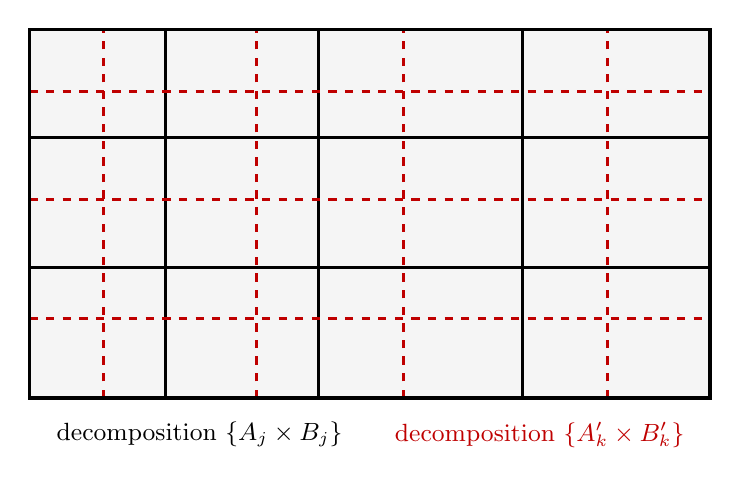
\begin{tikzpicture}[scale=0.72]
  \fill[black!4] (0,0) rectangle (12,6.5);
  % first decomposition: solid
  \foreach \x in {2.4,5.1,8.7} { \draw[line width=1.0pt] (\x,0) -- (\x,6.5); }
  \foreach \y in {2.3,4.6} { \draw[line width=1.0pt] (0,\y) -- (12,\y); }
  % second decomposition: dashed
  \foreach \x in {1.3,4.0,6.6,10.2} { \draw[red!75!black,dashed,line width=1.0pt] (\x,0) -- (\x,6.5); }
  \foreach \y in {1.4,3.5,5.4} { \draw[red!75!black,dashed,line width=1.0pt] (0,\y) -- (12,\y); }
  \draw[line width=1.3pt] (0,0) rectangle (12,6.5);
  \node[below] at (3,-0.25) {\small decomposition $\{A_j \times B_j\}$};
  \node[below,red!75!black] at (9,-0.25) {\small decomposition $\{A_k' \times B_k'\}$};
\end{tikzpicture}
\caption{Two different decompositions of the same rectangle into disjoint
sub-rectangles. Overlaying them gives a common refinement, on which both
values of $\pi$ can be computed and compared.}
\end{figure}

%---------------------------------------------------------------------
\subsection{\texorpdfstring{$\sigma$}{sigma}-Finiteness}
%---------------------------------------------------------------------

\begin{definition}[$\sigma$-finite]
A measure $\mu$ on a measurable space $(X,\M)$ is \emph{$\sigma$-finite}
if there exists a countable collection of sets
$\{E_j\}_{j=1}^{\infty} \subset \M$ such that
\[
  X = \bigcup_{j=1}^{\infty} E_j
  \qquad \text{and} \qquad
  \mu(E_j) < \infty \text{ for every } j.
\]
\end{definition}

In other words, $X$ can be covered by countably many sets of finite
measure, even if $\mu(X)$ itself is infinite.

\begin{example}
Lebesgue measure $m$ on $\R$ is $\sigma$-finite: taking
$E_j = (-j,j)$ for $j = 1,2,3,\ldots$ gives
\[
  \R = \bigcup_{j=1}^{\infty} (-j,j),
  \qquad m((-j,j)) = 2j < \infty,
\]
even though $m(\R) = \infty$.
\end{example}

%=====================================================================
\section{Sections}
%=====================================================================

%---------------------------------------------------------------------
\subsection{Sections of Sets}
%---------------------------------------------------------------------

Let $X$ and $Y$ be sets, and let $E \subset X \times Y$. For $x \in X$,
the \emph{$x$-section} of $E$ is the subset of $Y$ given by
\[
  E_x = \{ y \in Y : (x,y) \in E \}.
\]
Similarly, for $y \in Y$, the \emph{$y$-section} of $E$ is the subset
of $X$ given by
\[
  E^{y} = \{ x \in X : (x,y) \in E \}.
\]

Intuitively, $E_x$ is the ``slice'' of $E$ you get by fixing the first
coordinate at $x$ and looking at which $y$'s pair with it; $E^{y}$ is
the analogous slice fixing the second coordinate.

\begin{example}
If $E = A \times B$ is a rectangle, then
\[
  E_x = \begin{cases} B & \text{if } x \in A \\ \emptyset & \text{if } x \notin A \end{cases}
  \qquad \text{and} \qquad
  E^{y} = \begin{cases} A & \text{if } y \in B \\ \emptyset & \text{if } y \notin B. \end{cases}
\]
\end{example}

\begin{figure}[H]
\centering
\begin{tikzpicture}[scale=1.0]
  \draw[->] (0,0) -- (7.2,0) node[right] {$X$};
  \draw[->] (0,0) -- (0,4.6) node[above] {$Y$};
  \draw[line width=1.2pt]
    plot[smooth cycle,tension=0.85] coordinates
      {(1.6,2.0) (2.4,3.6) (3.9,3.9) (5.2,3.2) (5.6,1.9) (4.2,0.9) (2.6,0.85)};
  \draw (3.35,0.95) -- (3.35,3.78);
  \draw (1.72,2.45) -- (5.58,2.45);
  \node[above] at (3.35,3.8) {$E_x$};
  \node[right] at (5.62,2.45) {$E^{y}$};
  \draw (3.35,-0.1) -- (3.35,0.1);
  \node[below] at (3.35,-0.12) {$x$};
  \draw (-0.1,2.45) -- (0.1,2.45);
  \node[left] at (-0.12,2.45) {$y$};
\end{tikzpicture}
\caption{The $x$-section and $y$-section of a set $E \subset X \times Y$.}
\end{figure}

%---------------------------------------------------------------------
\subsection{Sections of Functions}
%---------------------------------------------------------------------

Let $f : X \times Y \to \Rbar$ (or $\mathbb{C}$) be a function. For
$x \in X$, the \emph{$x$-section} of $f$ is the function
$f_x : Y \to \Rbar$ defined by
\[
  f_x(y) = f(x,y).
\]
Similarly, for $y \in Y$, the \emph{$y$-section} of $f$ is the function
$f^{y} : X \to \Rbar$ defined by
\[
  f^{y}(x) = f(x,y).
\]

In words, $f_x$ is obtained by freezing the first coordinate at $x$ and
letting $y$ vary, while $f^{y}$ freezes the second coordinate and lets
$x$ vary. Note that
\[
  (f_x)(y) = (f^{y})(x) = f(x,y)
\]
for all $x \in X$, $y \in Y$ --- they are just two different ways of
slicing the same function.

\begin{figure}[H]
\centering
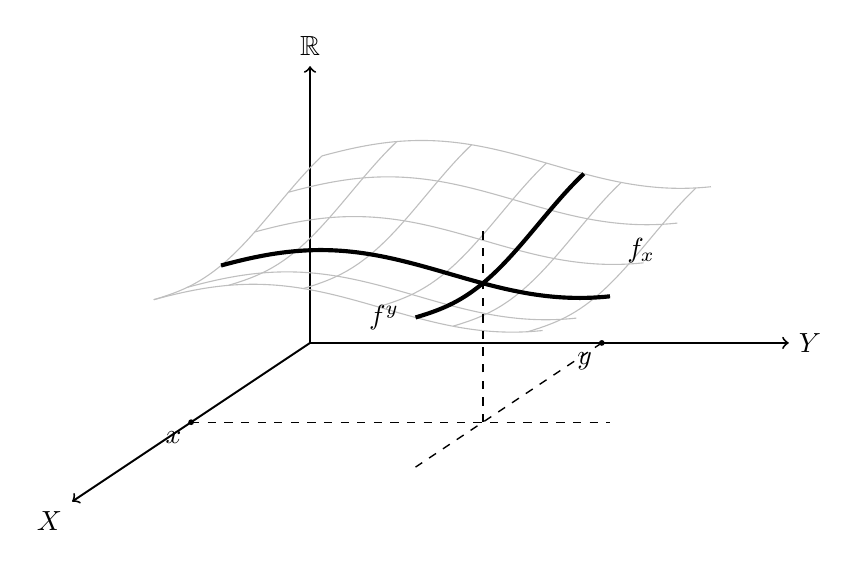
\begin{tikzpicture}[scale=0.95,
    x={(-0.60cm,-0.40cm)}, y={(1.00cm,0cm)}, z={(0cm,1.00cm)}]
  \draw[->,line width=0.7pt] (0,0,0) -- (5.3,0,0) node[below left] {$X$};
  \draw[->,line width=0.7pt] (0,0,0) -- (0,6.4,0) node[right] {$Y$};
  \draw[->,line width=0.7pt] (0,0,0) -- (0,0,3.7) node[above] {$\mathbb{R}$};
  \foreach \u in {0.4,1.15,1.9,2.65,3.4,4.15} {
    \draw[gray!50,line width=0.4pt] plot[domain=0.4:5.6,samples=50,smooth,variable=\v]
      ({\u},{\v},{2.35+0.32*sin(52*\v)+0.24*cos(64*\u)-0.05*\u});
  }
  \foreach \v in {0.4,1.4,2.4,3.4,4.4,5.4} {
    \draw[gray!50,line width=0.4pt] plot[domain=0.4:4.15,samples=40,smooth,variable=\u]
      ({\u},{\v},{2.35+0.32*sin(52*\v)+0.24*cos(64*\u)-0.05*\u});
  }
  \draw[line width=1.5pt] plot[domain=0.4:5.6,samples=60,smooth,variable=\v]
    ({2.65},{\v},{2.35+0.32*sin(52*\v)+0.24*cos(64*2.65)-0.05*2.65});
  \draw[line width=1.5pt] plot[domain=0.4:4.15,samples=50,smooth,variable=\u]
    ({\u},{3.9},{2.35+0.32*sin(52*3.9)+0.24*cos(64*\u)-0.05*\u});
  \node[right] at (2.65,5.7,2.30) {$f_x$};
  \node[below left] at (4.3,3.9,2.35) {$f^{y}$};
  \draw[dashed,line width=0.5pt] (2.65,0,0) -- (2.65,5.6,0);
  \draw[dashed,line width=0.5pt] (0,3.9,0) -- (4.15,3.9,0);
  \draw[dashed,line width=0.5pt] (2.65,3.9,0) -- (2.65,3.9,2.55);
  \fill (2.65,0,0) circle (1.1pt); \node[below left] at (2.65,0,0) {$x$};
  \fill (0,3.9,0) circle (1.1pt); \node[below left] at (0,3.9,0) {$y$};
\end{tikzpicture}
\caption{The graph of $f$ over $X \times Y$, with the section $f_x$ obtained
by freezing the first coordinate and the section $f^{y}$ obtained by freezing
the second.}
\end{figure}

%---------------------------------------------------------------------
\subsection{Sections and the Product Measure}
%---------------------------------------------------------------------

\begin{theorem}
Suppose $(X,\M,\mu)$ and $(Y,\N,\nu)$ are $\sigma$-finite measure
spaces. If $E \in \M \otimes \N$, then the functions
$x \mapsto \nu(E_x)$ and $y \mapsto \mu(E^{y})$ are measurable on $X$
and $Y$, respectively, and
\[
  \mu \times \nu(E)
    \;=\; \int \nu(E_x) \,d\mu(x)
    \;=\; \int \mu(E^{y}) \,d\nu(y).
\]
\end{theorem}

This is the statement that the measure of a set can be recovered by
integrating the sizes of its slices, and it is the set-level precursor
of the theorems in the next section.

%=====================================================================
\section{Tonelli's and Fubini's Theorems}
%=====================================================================

\begin{theorem}[Tonelli]
Suppose that $(X,\M,\mu)$ and $(Y,\N,\nu)$ are $\sigma$-finite measure
spaces. If $f \in L^{+}(X \times Y)$, then
\[
  \int f \,d(\mu \times \nu)
    \;=\; \int \left[ \int f(x,y) \,d\nu(y) \right] d\mu(x)
    \;=\; \int \left[ \int f(x,y) \,d\mu(x) \right] d\nu(y).
\]
\end{theorem}

\begin{theorem}[Fubini]
Suppose that $(X,\M,\mu)$ and $(Y,\N,\nu)$ are $\sigma$-finite measure
spaces. If $f \in L^{1}(\mu \times \nu)$, then $f_x \in L^{1}(\nu)$ for
a.e.\ $x \in X$, and $f^{y} \in L^{1}(\mu)$ for a.e.\ $y \in Y$, and
\[
  \int f \,d(\mu \times \nu)
    \;=\; \int \left[ \int f(x,y) \,d\nu(y) \right] d\mu(x)
    \;=\; \int \left[ \int f(x,y) \,d\mu(x) \right] d\nu(y).
\]
\end{theorem}

The two theorems differ only in their hypothesis on $f$: Tonelli
requires nonnegativity, Fubini requires absolute integrability. Neither
hypothesis can simply be dropped, as the next section shows.

%=====================================================================
\section{Why \texorpdfstring{$L^{1}$}{L1} is Necessary: A Counterexample to Fubini}
%=====================================================================

Define $f : [0,1]^{2} \to \R$ by
\[
  f(x,y) = \frac{x^{2} - y^{2}}{(x^{2} + y^{2})^{2}},
  \qquad (x,y) \ne (0,0), \qquad f(0,0) = 0.
\]

\noindent
\textbf{The iterated integrals both exist, but disagree.} One can
compute
\[
  \int_0^1 f(x,y) \,dy = \frac{1}{1+x^{2}}
  \quad \implies \quad
  \int_0^1 \left( \int_0^1 f(x,y) \,dy \right) dx
    = \int_0^1 \frac{dx}{1+x^{2}} = \frac{\pi}{4},
\]
while
\[
  \int_0^1 f(x,y) \,dx = \frac{-1}{1+y^{2}}
  \quad \implies \quad
  \int_0^1 \left( \int_0^1 f(x,y) \,dx \right) dy
    = \int_0^1 \frac{-dy}{1+y^{2}} = -\frac{\pi}{4}.
\]
So
\[
  \int_0^1 \left( \int_0^1 f(x,y) \,dy \right) dx
    = \frac{\pi}{4}
    \;\ne\; -\frac{\pi}{4}
    = \int_0^1 \left( \int_0^1 f(x,y) \,dx \right) dy.
\]

\noindent
\textbf{Why Fubini doesn't apply.} One can check that
\[
  \iint_{[0,1]^{2}} |f(x,y)| \,d(x,y) = \infty,
\]
so $f \notin L^{1}([0,1]^{2}, m \times m)$. The hypothesis of Fubini's
theorem fails, and indeed its conclusion fails: the two iterated
integrals, though individually well-defined and finite, are not equal.

\medskip
\noindent
\textbf{Moral.} Absolute integrability over the product space is not a
technicality --- without it, the order of integration can genuinely
matter.

%=====================================================================
\begin{thebibliography}{9}
\bibitem{folland}
  G.~B. Folland,
  \emph{Real Analysis: Modern Techniques and Their Applications},
  2nd ed., Wiley, 1999.

\bibitem{tao}
  T.~Tao,
  \emph{An Introduction to Measure Theory},
  Graduate Studies in Mathematics, vol.~126,
  American Mathematical Society, 2011.
\end{thebibliography}

\end{document}